\documentclass[11pt]{article}
\usepackage[margin=1in]{geometry}
\usepackage{graphicx}
\usepackage{booktabs}
\usepackage{hyperref}
\usepackage{siunitx}
\usepackage{float}
\usepackage{caption}
\usepackage{subcaption}
\usepackage{enumitem}

\title{Checkpoint 2: Baseline Model and Results\\CPSC 4300/6300 Applied Data Science}
\author{Michael Joseph Ellis}
\date{\today}

\begin{document}
\maketitle

\section*{Model Choice and Rationale}
We frame the task as multi-class classification of \texttt{GradeClass} (0=A, 1=B, 2=C, 3=D, 4=F). Guided by our EDA, we select gradient-boosted decision trees (XGBoost)\footnote{XGBoost documentation: \url{https://xgboost.readthedocs.io}. Chen \& Guestrin (2016): \url{https://arxiv.org/abs/1603.02754}.} because they:
\begin{itemize}[leftmargin=*]
  \item handle mixed numeric/categorical inputs and non-linear feature interactions;
  \item are robust to monotone transformations and outliers in features like \texttt{Absences};
  \item provide useful diagnostics (feature importance, confusion matrices) for interpretation.
\end{itemize}
We use \texttt{objective=multi:softprob}, \texttt{tree\_method=hist}, and native categorical support (integer-coded categories). We drop \texttt{StudentID} and \texttt{GPA} to avoid identifier leakage and using the continuous target precursor.

\section*{Evaluation Protocol}
We reserve 20\% of the data as a held-out test set with stratification (random seed 42). On the remaining 80\% training portion, we estimate baseline generalization via 5-fold \emph{StratifiedKFold} cross-validation with shuffling, scored by macro-averaged F1 (macro-F1) to account for class imbalance (many F's). Importantly, cross-validation is performed strictly within the training split; the test set remains untouched until the very end.

For model training, we further carve out a small validation split from the training data (again stratified) that is used only to monitor training; we do not perform hyperparameter tuning in this baseline. Features require no scaling for tree models. Categorical predictors are provided as pandas \texttt{category} dtype to XGBoost's native categorical handling, while \texttt{StudentID} and \texttt{GPA} are dropped to prevent target leakage.

We report: (i) cross-validated macro-F1 on the training split; (ii) held-out test accuracy and macro-F1; (iii) per-class precision/recall/F1 via \texttt{classification\_report}; and (iv) both raw-count and row-normalized confusion matrices for qualitative error analysis. Predicted labels are taken as \texttt{argmax} over \texttt{multi:softprob} outputs; the ``confidence'' used in examples is that maximum class probability.

\section*{Results}
\textbf{Cross-Validation (train split):} macro-F1 $=0.566\,\pm\,0.057$.

\textbf{Held-out Test:} Accuracy $=0.658$, macro-F1 $=0.487$.

Per-class precision/recall/F1 on the test set (labels map to A,B,C,D,F):
\begin{center}
\sisetup{round-mode=places,round-precision=3}
\begin{tabular}{l S S S S}
\toprule
Class & {Precision} & {Recall} & {F1} & {Support} \\
\midrule
A (0) & 0.308 & 0.190 & 0.235 & 21 \\
B (1) & 0.471 & 0.444 & 0.457 & 54 \\
C (2) & 0.447 & 0.487 & 0.466 & 78 \\
D (3) & 0.379 & 0.398 & 0.388 & 83 \\
F (4) & 0.889 & 0.889 & 0.889 & 243 \\
\midrule
Macro avg & 0.499 & 0.482 & 0.487 & 479 \\
Weighted avg & 0.656 & 0.658 & 0.656 & 479 \\
\bottomrule
\end{tabular}
\end{center}

\section*{Visualizations}
\begin{figure}[H]
  \centering
  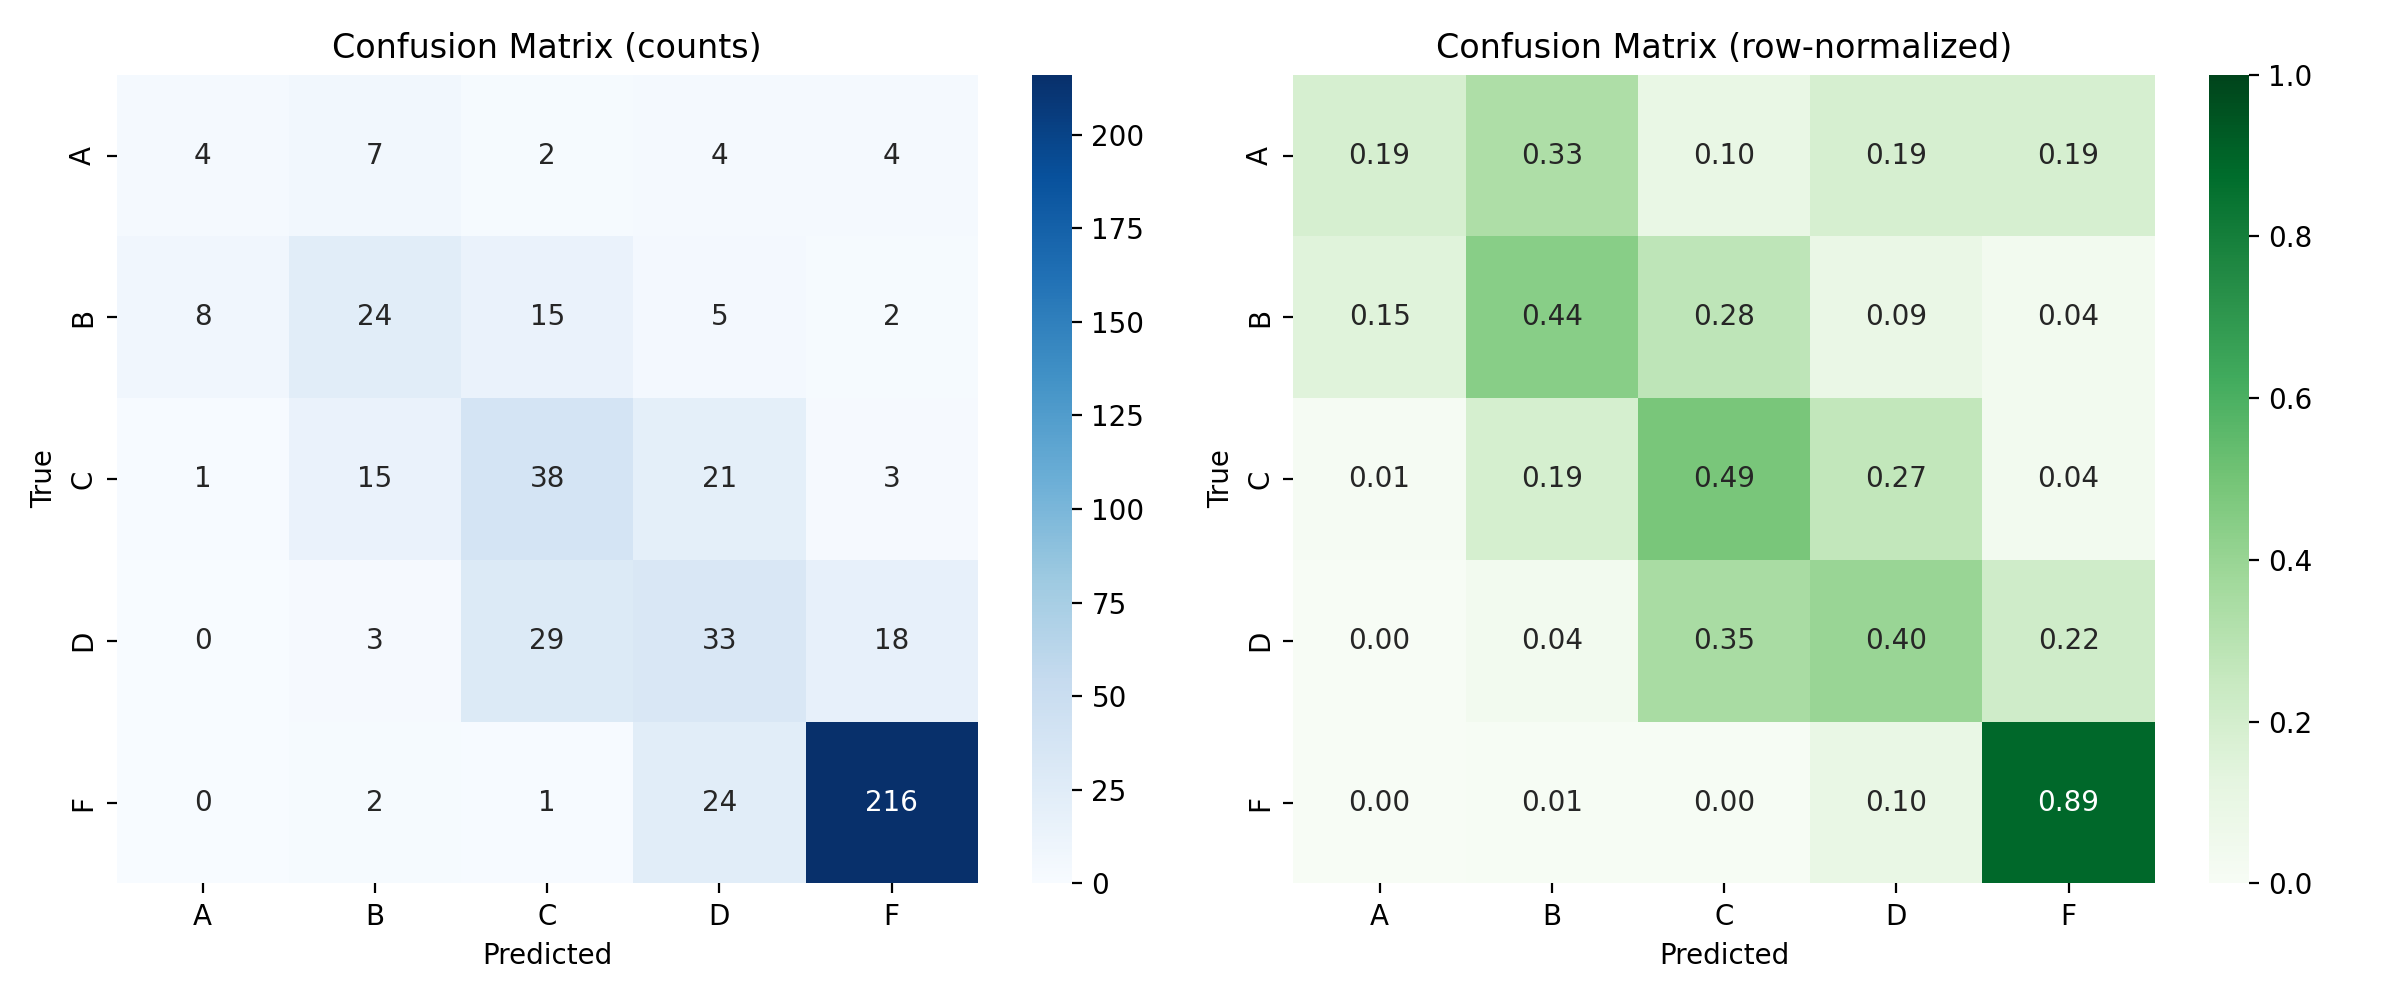
\includegraphics[width=.9\textwidth]{../Checkpoint 2/figures/xgb_confusion_mats.png}
  \caption{Confusion matrices (counts and row-normalized) for the held-out test set.}
\end{figure}

\begin{figure}[H]
  \centering
  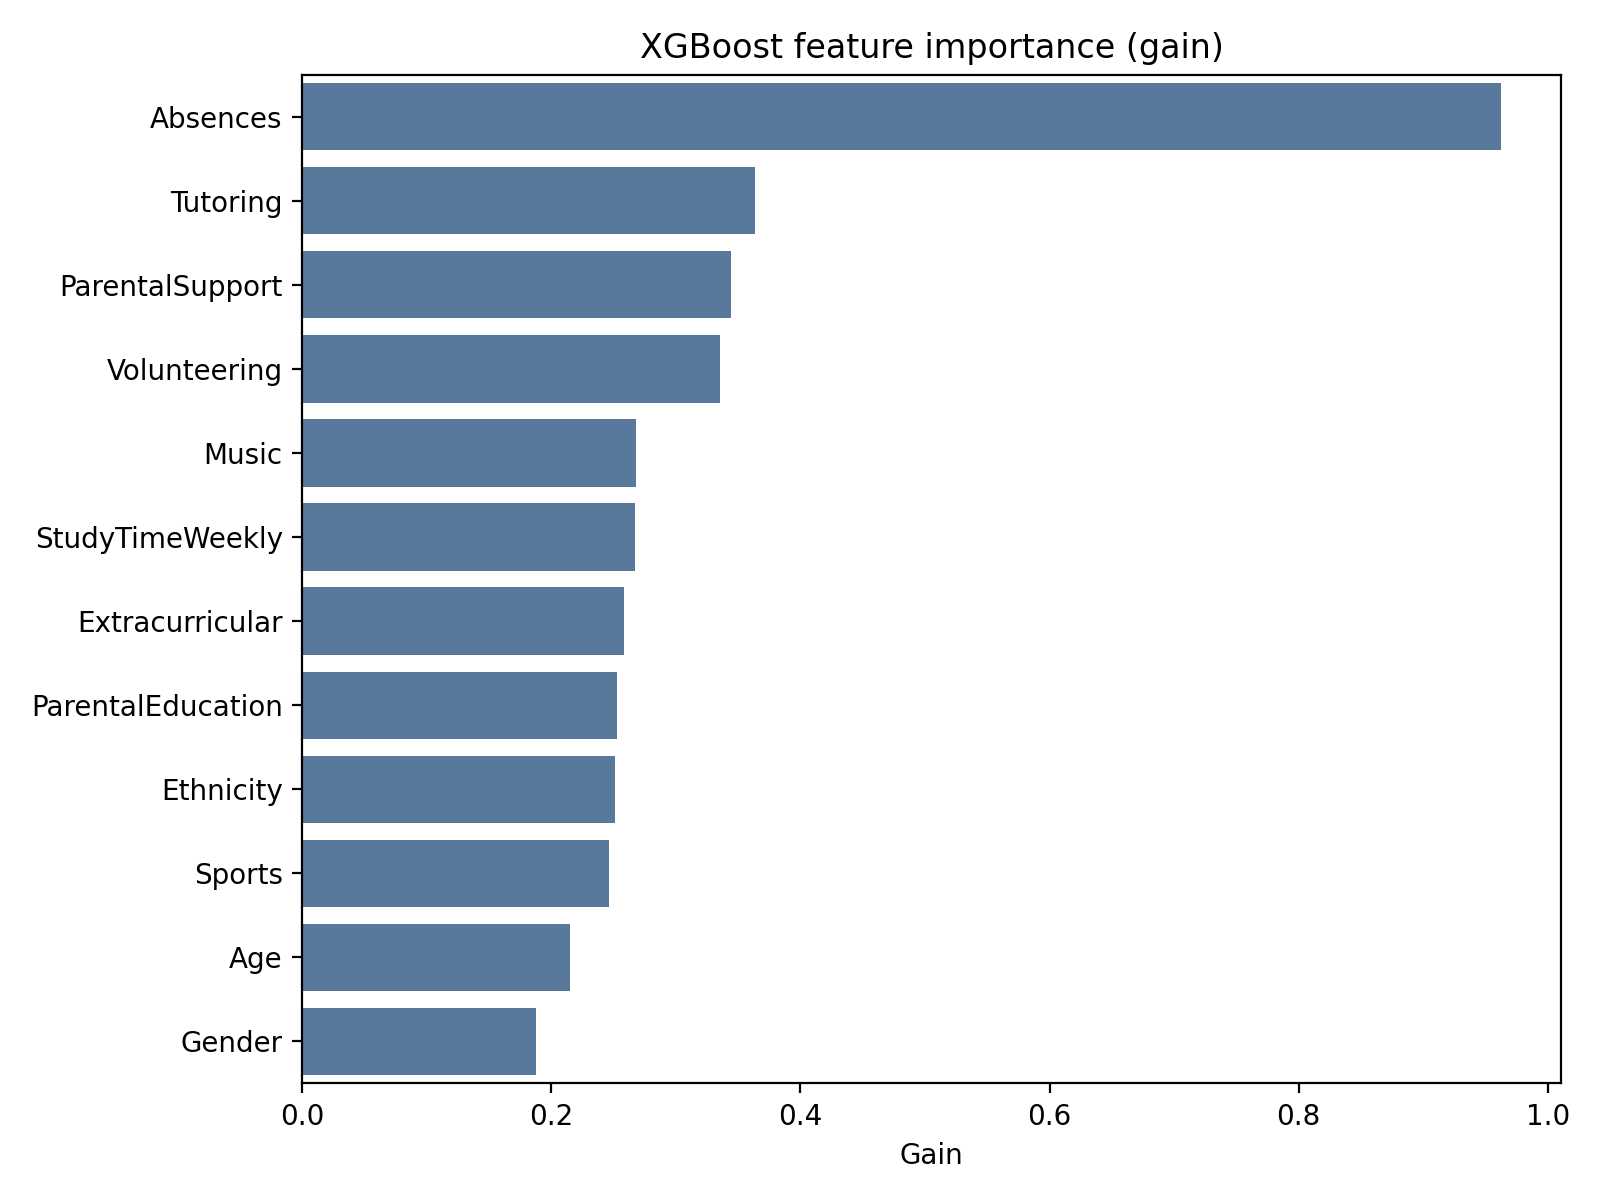
\includegraphics[width=.8\textwidth]{../Checkpoint 2/figures/xgb_feature_importance.png}
  \caption{XGBoost feature importance (gain).}
\end{figure}

\section*{Discussion}
Overall accuracy is driven by strong performance on the majority class F (precision/recall $\approx 0.89$), while performance on minority classes (A/B) is notably weaker---a pattern consistent with the class imbalance seen in EDA. Macro-F1, which weights each class equally, therefore lands below accuracy. The confusion matrices indicate that most errors occur between ``neighboring'' grades (e.g., A vs. B, C vs. D), suggesting the features capture broad achievement bands but struggle to separate adjacent boundaries.

From an interpretability angle, the feature-importance plot provides directional insight into which signals the model finds most useful. While tree-based gain does not establish causality, it helps prioritize follow-up analysis and potential feature engineering (e.g., interaction or monotonic constraints if justified by domain knowledge). Because outputs are uncalibrated probabilities, users should be cautious interpreting the magnitude of predicted confidence; if calibrated decision support is desired, post-hoc calibration (isotonic or Platt scaling) on a validation set would be appropriate.

Clear, incremental next steps include:
\begin{itemize}[leftmargin=*]
  \item \textbf{Class sensitivity:} incorporate per-class sample weights (e.g., inverse-frequency) to reduce bias toward F; optionally explore focal loss or custom loss.
  \item \textbf{Hyperparameter tuning:} a small search over depth, learning rate, trees, subsampling, and regularization to improve macro-F1 while guarding against overfit.
  \item \textbf{Decision policy:} if the use case prioritizes early risk identification, optimize metrics aligned to that objective (e.g., recall for D/F) or set class-specific thresholds.
  \item \textbf{Calibration:} apply probability calibration if thresholds or risk scores will be acted on by advisors or automated systems.
  \item \textbf{Feature refinement:} engineer richer engagement signals (e.g., attendance trends, interaction terms) if available, and reassess importance and confusion patterns.
\end{itemize}

\section*{Example Predictions (Three Cases)}
We include three high-confidence predictions from the test set, aiming to illustrate success and borderline cases. ``Index'' refers to the row index within the test split (not \texttt{StudentID}). ``Confidence'' is the model's maximum predicted probability for the predicted class. We deliberately select one predicted A, one predicted B, and one predicted F when available.

\begin{center}
\begin{tabular}{l l l l}
\toprule
Index & True & Pred & Confidence \\
\midrule
475 & B & A & 0.999 \\
118 & A & B & 0.998 \\
464 & F & F & 1.000 \\
\bottomrule
\end{tabular}
\end{center}

Brief interpretation: the B$\to$A and A$\to$B flips are typical boundary confusions where the available features do not cleanly separate adjacent top grades; despite very high confidence, such cases highlight the need for probability calibration if confidence will drive actions. By contrast, the F$\to$F prediction reflects a pattern the model recognizes reliably on this dataset, aligning with strong test-set precision/recall for F. In practice, pairing these probabilities with decision thresholds tuned to institutional goals (e.g., flagging at-risk students) is recommended.

\section*{Reproducibility}
Artifacts produced by \texttt{data analysis/models/xgb\_baseline.py}:
\begin{itemize}[leftmargin=*]
  \item Figures: \texttt{Checkpoint 2/figures/xgb\_confusion\_mats.png}, \texttt{Checkpoint 2/figures/xgb\_feature\_importance.png}
  \item Summary JSON: \texttt{Checkpoint 2/xgb\_baseline\_summary.json}
  \item Three cases: \texttt{Checkpoint 2/xgb\_three\_cases.csv}
\end{itemize}
Run with Python 3.11 virtual environment (Windows PowerShell):
\begin{verbatim}
.\.venv311\Scripts\python.exe ".\data analysis\models\xgb_baseline.py"
\end{verbatim}

\vspace{.5em}
\noindent\textbf{References:}
\begin{itemize}[leftmargin=*]
  \item XGBoost Documentation: \url{https://xgboost.readthedocs.io/en/stable/}
  \item Chen, T., \& Guestrin, C. (2016). XGBoost: A Scalable Tree Boosting System. \emph{arXiv:1603.02754}.
\end{itemize}

\end{document}
